\documentclass[11pt,spanish,a4paper]{article}
% Versión 1er cuat 2015 Víctor Bettachini < bettachini@df.uba.ar >

\usepackage{babel}
\addto\shorthandsspanish{\spanishdeactivate{~<>}}
\usepackage[utf8]{inputenc}
\usepackage{float}
\usepackage{units}
\usepackage{siunitx}
\usepackage{amsmath}
\usepackage{amstext}
\usepackage{amssymb}
\usepackage{graphicx}
\graphicspath{ {./graphs/} {../}}

\voffset-3.5cm
\hoffset-3cm
\setlength{\textwidth}{17.5cm}
\setlength{\textheight}{27cm}

\usepackage{lastpage}
\usepackage{fancyhdr}
\pagestyle{fancyplain}
\fancyhead{}
\fancyfoot{{\tiny \textcopyright Departamento de Física, FCEyN, UBA}}
\fancyfoot[C]{ {\tiny Actualizado al \today} }
\fancyfoot[RO, LE]{Pág. \thepage/\pageref{LastPage}}
\renewcommand{\headrulewidth}{0pt}
\renewcommand{\footrulewidth}{0pt}


\begin{document}
\begin{center}
	\textsc{\large Física 2 (Físicos)} - Prof. Hernán Grecco - 1"er cuat. 2015\\
	\textsc{\large Guía 4:}	Otras ecuaciones de ondas
\end{center}

\begin{enumerate}
\item Encuentre los modos normales de la cuerda ilustrada en la figura, que está sujeta fija en sus extremos y tiene una masa sujetada en el centro.
\begin{center}
	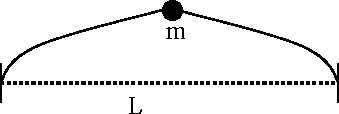
\includegraphics[width=0.25\linewidth]{g04e01}
\end{center}


\item Se establece una onda sonora estacionaria en el interior de un tubo de 1m de longitud \SI{5}{cm} de diámetro.
	Si se la excita en el modo más bajo con una presión pico de \SI{d-7}{N/cm^2}, calcule el desplazamiento pico y el cambio de densidad pico, así como la energía total contenida en la onda confinada en el tubo.
	Haga el cálculo para el tubo cerrado en ambos extremos y para el tubo abierto en un extremo.
	Compare ese desplazamiento con la distancia media entre moléculas en el aire.
	Nota: el ejemplo dado corresponde a un sonido apenas audible.


\item Un resorte con extremos libres es comprimido inicialmente un 5\% en su 10\% central y se lo suelta.
	Escriba las condiciones iniciales, halle su descomposición en modos normales y escriba la solución para todo tiempo.
	Demuestre que la solución es periódica (¿con qué periodo?) y dibuje (con ayuda de una computadora) la solución para 10 tiempos distintos dentro de un periodo.
	Discuta el resultado.
\begin{center}
	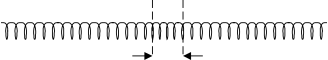
\includegraphics[width=0.35\linewidth]{g04e03}
\end{center}


\item Un resorte apoyado horizontalmente sin rozamiento y fijo en un extremo, tiene una masa \(M\) sujeto en el otro extremo.
	Calcule los modos normales de oscilación longitudinal del resorte.
\begin{center}
	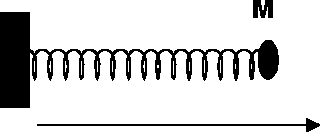
\includegraphics[width=0.2\linewidth]{g04e04}
\end{center}


\item Una barra cuelga soldada a un alambre de torsión (similar al caso del ejercicio 1 de la guía 2) con el otro extremo libre para girar.
	Encuentre los modos de torsión del alambre.
	Repita el cálculo para el extremo del alambre fijo.
\begin{center}
	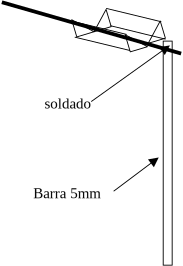
\includegraphics[width=0.15\linewidth]{g04e05}
\end{center}



\item Utilizando el resultado anterior y consideraciones de simetría resuelva el ejercicio 1 de la guía 2 teniendo en cuenta las ondas de torsión que se propagan por el alambre.
	Compare los modos mas bajos con la solución hallada para el mencionado caso en que se consideró como de dos grados de libertad.


\item Se tiene un sistema de masas acopladas por resortes.
	Halle la ecuación de ondas correspondiente a las oscilaciones longitudinales y transversales despreciando la masa de los resortes.
	Encuentre la relación de dispersión para este sistema y grafíquela.
\begin{center}
	
\includegraphics[width=0.25\linewidth]{g04e07}
\end{center}


\item Se tiene un sistema de péndulos acoplados longitudinalmente por resortes.
	Halle la ecuación de ondas correspondiente a las oscilaciones longitudinales y transversales despreciando la masa
	de los resortes.
	Encuentre la relación de dispersión para este sistema y grafíquela.
\begin{center}
	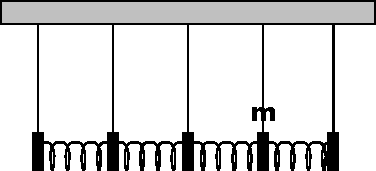
\includegraphics[width=0.25\linewidth]{g04e08}
\end{center}


\item Para el problema anterior resuelva para el caso en que las \(\omega< \omega_\mathrm{min}\) o \(\omega> \omega_\mathrm{max} \).
		Para ello proponga una solución del tipo \(A_n= A \mathrm{e}^{\pm kan} \), y encuentre la nueva relación entre \(\omega\) y su correspondiente \(k\) complejo.

\end{enumerate}
\end{document}
